\chapter{3. Singleton Pattern}

\section{Giới thiệu}
\subsection{Đặt vấn đề}
Hầu hết các đối tượng trong một ứng dụng đều chịu trách nhiệm cho công việc của chúng và truy xuất dữ liệu tự lưu trữ (self-contained data) với các tham chiếu trong phạm vi được đưa ra. Tuy nhiên, có nhiều đối tượng có thêm những nhiệm vụ và có ảnh hưởng rộng hơn, chẳng hạn như quản lý các nguồn tài nguyên bị giới hạn hoặc theo dõi toàn bộ trạng thái của hệ thống. Ví dụ có nhiều máy in trong một hệ thống nhưng chỉ tồn tại duy nhất một Sprinter Spooler (Phần quản lí máy in).\\
Hay giả sử trong ứng dụng có chức năng bật tắt nhạc nền chẳng hạn, khi người dùng mở app thì ứng dụng sẽ tự động mở nhạc nền và nếu người dùng muốn tắt thì phải vào setting trong app để tắt nó, trong setting của app cho phép người dùng quản lí việc mở hay tắt nhạc, và trong trường hợp này sẽ cần sử dụng singleton để quản lí. Chắc chắn chúng ta phải cần duy nhất 1 instance để có thể ra lệnh bật hay tắt, tại sao? Vì đơn giản bạn không thể tạo 1 instance để mở nhạc rồi sau đó lại tạo 1 instance khác để tắt nhạc, lúc này sẽ có 2 instance được tạo ra, 2 instance này không liên quan đến nhau nên không thể thực hiện thực hiện việc cho nhau được. Nói cách khác instance nào bật thì chỉ có instance đó mới được phép tắt nên dẫn đến phải cần 1 instance.\\
Để phục vụ nhu cầu kể trên Singleton Pattern đã được tạo ra.
\subsection{Mục đích sử dụng}
Mô hình thiết kế singleton giải quyết các vấn đề bằng cách cho phép nó:
\begin{itemize}
    \item Đảm bảo rằng một class chỉ có một instance
    \item Dễ dàng truy cập instance duy nhất của một class
    \item Kiểm soát sự khởi tạo của instance
    \item Hạn chế số lượng phiên bản
    \item Truy cập một biến toàn cục
\end{itemize}
Mô hình thiết kế singleton mô tả cách giải quyết các vấn đề như:
\begin{itemize}
    \item Ẩn các constructor của một class .
    \item Định nghĩa một hoạt động tĩnh công khai ( getInstance()) trả về thể hiện duy nhất của class.
\end{itemize}

Về bản chất, mô hình Singleton buộc nó phải chịu trách nhiệm đảm bảo rằng nó chỉ được khởi tạo một lần. Một phương thức khởi tạo ẩn — được khai báo private hoặc protected đảm bảo rằng lớp không bao giờ có thể được khởi tạo từ bên ngoài lớp. Hoạt động tĩnh công cộng có thể được truy cập bằng cách sử dụng tên class và tên operation.\\Ví dụ Singleton.getInstance():.

\section{Định nghĩa và mô hình cấu trúc}

\subsection{Định nghĩa}
Singleton là một Design Pattern thuộc nhóm khởi tạo (Creational).Nó đảm bảo rằng một class chỉ có duy nhất một instance được khởi tạo và chỉ có một cách để có quyền truy cập vào instance đó.

\subsection{Mô hình cấu trúc}
\begin{figure}[!htb]
    \centering
    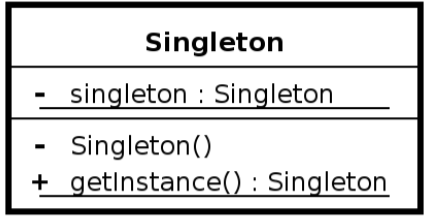
\includegraphics[height=6cm,width=9cm] {fig/Singleton/structure_singleton.png}
    \caption{Mô hình cấu trúc Singleton Pattern}
    \label{fig:structure_singleton}
\end{figure}

- Singleton chỉ liên quan đến một lớp duy nhất (thường không được gọi là Singleton). Lớp đó là một lớp đầy đủ với các thuộc tính và phương thức khác (không được hiển thị).
    
- Lớp có một biến static trỏ đến một thể hiện duy nhất của lớp.
    
- Lớp có một phương thức khởi tạo riêng (để ngăn mã khác khởi tạo lớp) và một phương thức tĩnh cung cấp quyền truy cập vào cá thể đơn lẻ.

\section{Cách cài đặt}
\subsection{Cài đặt chung}
Để cài đặt Singleton Pattern chúng ta cần làm hai bước.\\
Bước 1: Cần để class có duy nhất một instance
\begin{itemize}
    \item Private constructor của class đó để đảm bảo rằng class khác không thể truy cập vào constructor và tạo ra instance mới.
    \item Tạo một biến private static là thể hiện của class đó để đảm bảo rằng nó là duy nhất và chỉ được tạo ra trong class đó thôi.
\end{itemize}
Bước 2: Cung cấp một cách toàn cầu để truy cập tới instance đó
\begin{itemize}
    \item Tạo một public static method trả về instance vừa khởi tạo bên trên, đây là cách duy nhất để class khác có thể truy cập vào instance của class này.
\end{itemize}

Dưới đây là code minh họa cài đặt Singleton Pattern.

\begin{figure}[!htb]
    \centering
    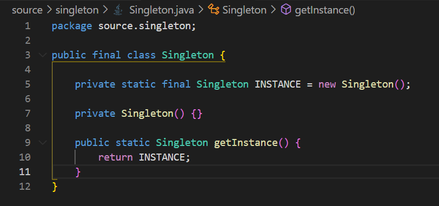
\includegraphics[width=\textwidth]
    {fig/Singleton/singleton_class.png}
    \caption{Singleton class}
    \label{fig:Singleton Class}
\end{figure}

\subsection{Cài đặt cho ví dụ cụ thể}
Dưới đây là ví dụ áp dụng Singleton Pattern.\\
Link code cài đặt:
\url{https://github.com/nanhus/OOP-DesginPatten/tree/master/source/singleton}

\begin{figure}[!htb]
    \centering
    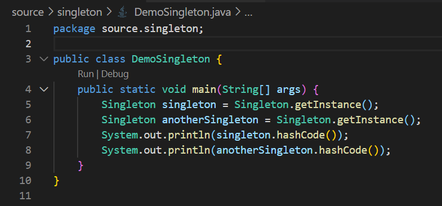
\includegraphics[width=\textwidth]{fig/Singleton/demo_singleton_class.png}
    \caption{Demo Singleton Class}
    \label{fig:demo_singleton_class}
\end{figure}
\begin{figure}[!htb]
    \centering
    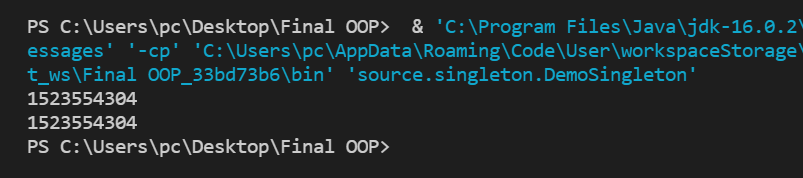
\includegraphics[width=\textwidth]{fig/Singleton/singleton_output.png}
    \caption{Output}
    \label{fig:singleton_output}
\end{figure}
\newpage
Như chúng ta đã thấy output cho ra kết quả là 2 ô nhớ cùng địa chỉ.Như vậy Singleton Pattern đã được cài đặt.

\section{Ví dụ thực tế}
\begin{itemize}
    \item Centralized manager of resources
    \begin{itemize}
        \item Window manager
        \item File system manager
        \item ...
    \end{itemize}
    \item Logger classes
    \item Factories
    \begin{itemize}
        \item Đặc biệt là những vấn đề  IDs
        \item Singleton thường được kết hợp với các mẫu Factory Method và Abstract Factory
    \end{itemize}
\end{itemize}

\newpage
